\documentclass[12pt]{amsart}
\usepackage{graphicx}
\usepackage{amssymb}
\usepackage{amsthm}
\usepackage{tikz}
\usepackage{multicol}
\usepackage{color}

\newcommand{\HRule}{\rule{\linewidth}{0.5mm}}
\def \red{\textcolor{red}}

\newtheorem*{theorem}{Theorem}
\newtheorem*{lemma}{Lemma}
\theoremstyle{definition}
\newtheorem*{definition}{Definition}

\begin{document}
  \begin{titlepage}
  \centering
  
  \huge{\textbf{Runge-Kutta Methods with Rooted Trees}}
  \\[0.1cm]
  \HRule
  \vfill
  
%\begin{multicols}{4}
%  \begin{center}
%  	\begin{tikzpicture}[baseline=0cm]
%	\node at (0,-0.6)  {$\bullet$};
%	\end{tikzpicture}
%  \end{center}
% 
% \begin{center}
%  	\begin{tikzpicture}[baseline=0cm]
%	\node at (0,-0.6)  {$\bullet$};
%	\node at (0,0)  {$\bullet$};
%	\draw (0,-0.6)--(0,0);
%	\end{tikzpicture}
%  \end{center}
%  
%  \begin{center}
%  	\begin{tikzpicture}[baseline=0cm]
%	\node at (-0.6,0)  {$\bullet$};
%	\node at (0.6,0)  {$\bullet$};
%	\node at (0,-0.6)  {$\bullet$};
%	\draw (0,-0.6)--(-0.6,0);
%	\draw (0,-0.6)--(0.6,0);
%	\end{tikzpicture}
%  \end{center}
%  
%  \begin{center}
%  	\begin{tikzpicture}[baseline=0cm]
%	\node at (-0.6,0)  {$\bullet$};
%	\node at (0,0)  {$\bullet$};
%	\node at (0.6,0)  {$\bullet$};
%	\node at (0,-0.6)  {$\bullet$};
%	\draw (0,-0.6)--(-0.6,0);
%	\draw (0,-0.6)--(0,0);
%	\draw (0,-0.6)--(0.6,0);
%	\end{tikzpicture}
%  \end{center}
%\end{multicols}
%\begin{multicols}{4}
%\begin{center}
%  	\begin{tikzpicture}[baseline=0cm]
%	\node at (0,-1.6)  {$\bullet$};
%	\node at (0,-0.8)  {$\bullet$};
%	\node at (0,0)  {$\bullet$};
%	\draw (0,-1.5)--(0,-0.8);
%	\draw (0,-0.8)--(0,0);
%	\end{tikzpicture}
%  \end{center}
%  
%\begin{center}
%  	\begin{tikzpicture}[baseline=0cm]
%	\node at (0,-1.5)  {$\bullet$};
%	\node at (0,-1.0)  {$\bullet$};
%	\node at (0,-0.5)  {$\bullet$};
%	\node at (0,0)  {$\bullet$};
%	\draw (0,-1.5)--(0,-1.0);
%	\draw (0,-1.0)--(0,-0.5);
%	\draw (0,-0.5)--(0,0);
%	\end{tikzpicture}
%  \end{center}
%  
%  \begin{center}
%  	\begin{tikzpicture}[baseline=0cm]
%	\node at (0,-1.6)  {$\bullet$};
%	\node at (0,-0.8)  {$\bullet$};
%	\node at (-0.5,0)  {$\bullet$};
%	\node at (0.5,0)  {$\bullet$};
%	\draw (0,-1.6)--(0,-0.8);
%	\draw (0,-0.8)--(-0.5,0);
%	\draw (0,-0.8)--(0.5,0);
%	\end{tikzpicture}
%  \end{center}
%  \begin{center}
%  	\begin{tikzpicture}[baseline=0cm]
%	\node at (0,-0.75)  {$\bullet$};
%	\node at (-0.5,0)  {$\bullet$};
%	\node at (0.5,0)  {$\bullet$};
%	\node at (-0.5,0.75)  {$\bullet$};
%	\draw (0,-0.75)--(-0.5,0);
%	\draw (0,-0.75)--(0.5,0);
%	\draw (-0.5,0)--(-0.5,0.75);
%	\end{tikzpicture}
%  \end{center}
%  
%\end{multicols}

  \vfill
  \textsc{\large Wilfrid Laurier University}
  \\[0.1cm]
  \textsc{\large MA489 Final Report}
  \HRule
  \\[0.5cm]
  
  \large \emph{Author:}
  \hfill
  \hfill
  \large \emph{Supervisor:}
  \\
  \large \textbf{Richard Douglas}
  \hfill
  \hfill
  \large \textbf{Dr. Shengda Hu}
  \\[2.0cm]
  \today{}
  \end{titlepage}
  
  \section{Introduction}
  This report picks up where the preceding interim report left off. It begins with some details that ensure the
  relevant basics of rooted trees are fully covered. What follows is some discussion regarding
  how the rooted tree approach of deriving the explicit Runge-Kutta methods works and more importantly, why it works. 
  The explicit third order Runge-Kutta methods with 3 stages are then derived. There is then some discussion
  of some simplifying assumptions that can be made in deriving methods of higher order. These assumptions are
  used in deriving the explicit methods of order 4 with 4 stages. 
  
  The report concludes by reproducing the numerical results obtained in a research article authored by \textit{Yao, Lai, and Li}
  where a Runge-Kutta method was used in solving a problem related to financial mathematics 
  (that is, deriving the efficient frontier in a general asset-liability model with endogenous liabilities). 
  See the accompanying Maple files for more details regarding how this was done.
  In closing, there are some remarks regarding numerical stability and why the implicit Runge-Kutta methods may also be of interest. 
  
  \section{Overview of the Derivation}
  The rooted tree approach of deriving Runge-Kutta methods works for the initial value problem
  $$y'(x) = f(y(x)) \mbox{ for all } x \in \left[ a, b \right]$$ 
  $$y(x_0) = y_0 \mbox{ for some } x_0 \in \left[ a, b \right]$$
  Here $y$ can be a vector-valued function of $x$ so this problem includes the scalar case in the preceding interim report 
  where $y'(x) = f(x,y)$.
  
  \noindent This is because we can let $$y^*(x) = \left( 
  \begin{tabular}{c}
  $x$ \\
  $y(x)$ \\
  \end{tabular} \right)$$ so that $$y^{*'}(x) = \left( 
  \begin{tabular}{c}
  $1$ \\
  $f(x,y(x))$ \\
  \end{tabular} \right) = f(y^*(x))$$
  
  The derivation works by making use of the fact that the corresponding Taylor method of order $p$
  $$y_{n+1} = y_n + f(y_n)h + f'(y_n)\frac{h^2}{2!} + \dots + f^{(p)}(y_n)\frac{h^{p}}{p!}$$
  and the Runge-Kutta approximation with $s$ stages
  $$y_{n + 1} = y_n + b_1hf(Y_1) + b_2hf(Y_2) + \dots + b_shf(Y_s)$$
  can be expressed in terms of rooted trees.
  
  \section{Denoting Rooted Trees}
   A rooted tree with a single vertex, that is, a tree with a root vertex and nothing else, is denoted by $\tau$.
  \begin{center}
	 \begin{tikzpicture}[baseline=0cm]
	\node at (0,0)  {$\bullet$};
	\end{tikzpicture}
  \end{center}
  Other rooted trees are denoted using a recursive notation. In general,
  $$\left[ t_1, t_2, \dots, t_m \right]$$
  denotes a rooted tree where the root has $m$ child nodes which form the respective subtrees $t_1, t_2, \dots, t_m$. 
  Since a subtree can show up more than once, it is convenient to use powers in the notation to indicate repetition. 
  An arbitrary rooted tree can also be represented as
  $$\left[ t^{m_1}_1, t^{m_2}_2, \dots, t^{m_n}_n \right]$$
  
   The letter $t$ is used to denote an arbitrary rooted tree. Recall that rooted trees that are isomorphic are
   treated as being equivalent. Isomorphism is an equivalence relation and thus each rooted tree belongs to its
   own respective equivalence class. A rooted tree $t$'s equivalence class with respect to isomorphism is known
   as its \textbf{abstract rooted tree} and is denoted by $|t|$. The set of all rooted trees is denoted $T$.   
  
  
  
  \section{Computing $\beta(t) \mbox{ and } \alpha(t)$}
  Recall that $\beta(t)$ measures the number of ways to label rooted tree $t$ such that
  labelings that indicate an automorphism are counted only once. Thus
  $$\beta(t) = \frac{r(t)!}{\sigma(t)}$$
  This is because a way to generate the $r(t)!$ ordinary labelings is to first choose a $\beta$
  labeling and then choose an automorphism. Thus $$\beta(t)\sigma(t) = r(t)!$$
  An expression for $\alpha(t)$ is
  $$\alpha(t) = \frac{r(t)!}{\sigma(t)\gamma(t)}$$
  The idea behind this expression is similar to the idea for $\beta(t)$ except this time we
  want to generate the $\beta$ labelings using the $\alpha$ labelings. Normally with $\beta$
  labelings we would have $r(t)$ choices for the root. With $\alpha$ labelings we are
  forced to choose the smallest label and thus only have 1 choice for the root's label.
  This is also true for the root of each subtree of $t$ and so
  $$\alpha(t)\gamma(t) = \beta(t) \implies \alpha(t) = \frac{\beta(t)}{\gamma(t)}$$
   
  \section{The Taylor Method in terms of Rooted Trees}
  The Taylor method is normally expressed in terms of the derivatives of $y$ (which are assumed to exist). 
  To get the derivatives in terms of rooted trees, we make use of the elementary differential. 
  
  \begin{definition} 
	Given a tree $t$ and a function $f : R^N \to R^N$ analytic in some
	neighbourhood of $y$, the \textbf{elementary differential} $F(t)(y)$ is defined
	recursively by
	$$F(\tau)(y) = f (y)$$
	$$F([t_1 ,t_2 ,...,t_m ])(y) = f^{(m)}(y)(F(t_1 )(y),F(t_2 )(y),...,F(t_m )(y))$$
  \end{definition}
  
  One interesting property of this rooted tree function is that rooted trees that belong
  to the same equivalence class share the same elementary differential.
  
  The rooted trees of order $\le 2$ and their elementary differentials are shown below
  \begin{multicols}{2}
  \begin{center}
    \begin{tikzpicture}[baseline=-0.25cm]
       \node at (0,-1)  {$\bullet$};
     \end{tikzpicture}
  \end{center}
  $$f(y)$$
  
  \begin{center}
  	\begin{tikzpicture}[baseline=-0.25cm]
	\node at (0,0)  {$\bullet$};
	\node at (0,1)  {$\bullet$};
	\draw (0,0)--(0,1);
	\end{tikzpicture}
  \end{center}
  $$f'(y)f(y)$$
\end{multicols}
Note that $$\frac{d}{dx}f(y(x)) = f'(y(x))f(y(x))$$

The rooted trees of order 3 with their elementary differentials are
\begin{multicols}{2}
    \begin{center}
  	\begin{tikzpicture}[baseline=-0.25cm]
	\node at (0,-2)  {$\bullet$};
	\node at (-1,-1)  {$\bullet$};
	\node at (1,-1)  {$\bullet$};
	\draw (0,-2)--(-1,-1);
	\draw (0,-2)--(1,-1);
	\end{tikzpicture}
  \end{center}
  $$f''(y)f(y)^2$$

  \begin{center}
    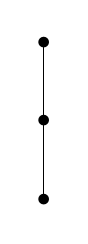
\begin{tikzpicture}[baseline=-0.25cm]
       \node at (0,0)  {$\bullet$};
       \node at (0,-1)  {$\bullet$};
       \node at (0,-2)  {$\bullet$};
       \draw (0,-2)--(0,-1);
       \draw (0,-1)--(0,0);
     \end{tikzpicture}
  \end{center}
  $$f'(y)^2f(y)$$
\end{multicols}
Similarly, $$\frac{d}{dx}f'(y(x))f(y(x)) = f''(y(x))f(y(x))^2 + f'(y(x))^2f(y(x))$$

\pagebreak
These examples provide motivation for the following lemma:
\begin{lemma}
Let $t$ be a rooted tree, then
$$\frac{d}{dx}F(|t|)(y)$$
is the sum of $F(u)(y)$ over all rooted trees $u$ such that if a leaf vertex is removed from $u$,
it becomes $t$.
\end{lemma}

\begin{proof}
The proof is by complete induction on the order of $t$ ($n = r(t)$). 
The base case is demonstrated in the preceding examples.  

let $t = \left[t_1, t_2, \dots t_m\right]$ and assume that the result holds for all trees with 
order strictly less than $r(t)$. 

Then
$$\frac{d}{dx}F(|t|)(y(x)) = \frac{d}{dx} f^{(m)}(y)(F(t_1)(y),F(t_2)(y), \dots, F(t_m)(y))$$
$$= f^{(m+1)}(y)(F(t_1)(y),F(t_2)(y), \dots, F(t_m)(y)) + Q_1 + Q_2 + \dots + Q_m$$
where 
$$Q_i = f^{(m)}(y)((F(t_1)(y),F(t_2)(y), \dots R_i, \dots, F(t_m)(y))$$
and
$$R_i = \frac{d}{dx}F(t_i)(y(x))$$
\hfill  $(\mbox{ for } i = 1, 2, \dots, m)$

Now $ f^{(m+1)}(y)(F(t_1)(y),F(t_2)(y), \dots, F(t_m)(y))$ corresponds to $t$ with an extra leaf 
protruding out of the root. Since $r(t_i) < r(t)$, the inductive hypothesis implies $R_i$ (and then $Q_i$) 
can be obtained by summing over the elementary differentials formed by inserting a leaf vertex to $t_i$.

Summing all the components together gives us the result. That is to say, the derivative of $F(t)(y(x))$ is 
the sum of the elementary differentials formed by inserting a leaf vertex to $t$. 
By complete induction, the lemma is proven.
\end{proof}
 An important thing to note about the lemma is that it is the  location
of the inserted leaf vertex that is summed over. It does not matter if two different locations
of the inserted leaf result in trees that are equivalent. 

Suppose for instance that we differentiate $F(\left[\tau^2\right])(y)$.
\begin{center}
  	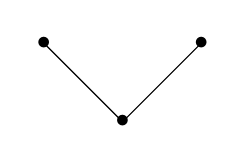
\begin{tikzpicture}[baseline=0cm]
	\node at (0,0)  {$\bullet$};
	\node at (-1,1)  {$\bullet$};
	\node at (1,1)  {$\bullet$};
	\draw (0,0)--(-1,1);
	\draw (0,0)--(1,1);
	\end{tikzpicture}
  \end{center}
  $$f''(y(x))f(y(x))^2$$
  Then there are $3$ rooted trees that can be formed by inserting a leaf vertex.
  \begin{multicols}{3}
   \begin{center}
  	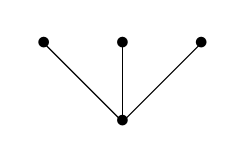
\begin{tikzpicture}[baseline=0cm]
	\node at (0,0)  {$\bullet$};
	\node at (-1,1)  {$\bullet$};
	\node at (0,1)  {$\bullet$};
	\node at (1,1)  {$\bullet$};
	\draw (0,0)--(-1,1);
	\draw (0,0)--(0,1);
	\draw (0,0)--(1,1);
	\end{tikzpicture}
	$$f'''(y)f(y)^3$$
  \end{center}
  
  \begin{center}
  	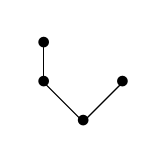
\begin{tikzpicture}[baseline=0cm]
	\node at (0,0)  {$\bullet$};
	\node at (-0.5,0.5)  {$\bullet$};
	\node at (0.5,0.5)  {$\bullet$};
	\node at (-0.5,1)  {$\bullet$};
	\draw (0,0)--(-0.5,0.5);
	\draw (0,0)--(0.5,0.5);
	\draw (-0.5,0.5)--(-0.5,1);
	\end{tikzpicture}
	$$f''(y)f'(y)f(y)^2$$
  \end{center}
  
\begin{center}
  	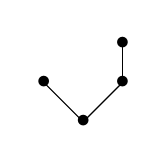
\begin{tikzpicture}[baseline=0cm]
	\node at (0,0)  {$\bullet$};
	\node at (-0.5,0.5)  {$\bullet$};
	\node at (0.5,0.5)  {$\bullet$};
	\node at (0.5,1)  {$\bullet$};
	\draw (0,0)--(-0.5,0.5);
	\draw (0,0)--(0.5,0.5);
	\draw (0.5,0.5)--(0.5,1);
	\end{tikzpicture}
	$$f''(y)f'(y)f(y)^2$$
  \end{center}
  \end{multicols}
  The second and third tree are equivalent but both are included in the sum of elementary differentials.
  $$\frac{d}{dx}f''(y(x))f(y(x))^2 = f'''(y)f(y)^3 + 2f''(y)f'(y)f(y)^2$$
  
  It turns out that there is a way to count the number of times a rooted tree's elementary differential
  will appear in the expression for the $k$th derivative of $y(x)$.
  \begin{theorem}
	Let $y(x)$ be a function such that $y'(x) = f(y(x))$, then assuming that it exists,
	$$y^{(k)}(x) = \sum_{r(|t|) = k}{\alpha(|t|)F(|t|)(y(x))}$$
	That is, the $k^{th}$ derivative of $y$ can be found by taking a representative of 
	each equivalence class from the set all rooted trees with $k$ vertices.
  \end{theorem}
  
  \begin{proof}
	By applying the preceding lemma repeatedly, it is clear that we will be summing all of the elementary differentials
	for the rooted trees of order $k$, however some elementary differentials will be appearing more than once. 
	This is where $\alpha(|t|)$ comes into play.

	An alternative way to interpret $\alpha(|t|)$ is as the number of ways in which you can start with a root vertex and
	``add vertices to the top'' so that $|t|$ is constructed. In fact, the $\alpha$ labelings tell us the valid orders in which 
	vertices can be chosen as the insertion location for the leaf vertex. 
	Recall that the labelings counted by $\alpha(|t|)$ are required to 
	assign each child vertex a higher label than its parent. This corresponds to how the parent vertex has to be
	inserted to the rooted tree construction before its children. $\alpha(|t|)$ also takes into account that in constructing $|t|$
	we do not care about the way that the insertion process is represented in a diagram, all that matters is the insertion locations
	and the order in which they are chosen (this corresponds to how $\alpha(|t|)$ treats two labelings that indicate
	an automorphism as being the same labeling).  
	
	Thus we know that the sum consists of the elementary differentials $F(|t|)(y)$  of each abstract rooted tree
	$|t|$ with $r(|t|) = k$ as well as how many times each term appears in the sum ($\alpha(|t|)$). 
	This gives us our result.
  \end{proof}
  
  With the derivatives of $y(x)$ taken care of, obtaining an expression for the Taylor method of order $p$ proves
  to be a simple task.
  
  \begin{theorem}
	The Taylor method of order $p$ can be written in terms of rooted trees as
	$$y_{n + 1} = y_n + \sum_{r(|t|) \le p}{\frac{h^{r(|t|)}}{\sigma(|t|)\gamma(|t|)}F(|t|)(y_n)}$$ 
  \end{theorem}
  \begin{proof}
  	 $$y_{n+1} = y_n + f(y_n)h + f'(y_n)\frac{h^2}{2!} + \dots + f^{(p)}(y_n)\frac{h^{p}}{p!}$$
  	 $$= y_n + \sum_{k = 1}^{p}{\frac{h^k}{k!}y^{(k)}(x_n)}$$
  	 $$= y_n + \sum_{k = 1}^{p}{\frac{h^k}{k!} \sum_{r(|t|) = k}{\alpha(|t|)F(|t|)(y_n)}}$$
  	 $$= y_n + \sum_{r(|t|) \le p}{\frac{h^{r(|t|)}\alpha(|t|)}{r(|t|)!}F(|t|)(y_n)}$$
  	 $$= y_n + \sum_{r(|t|) \le p}{\frac{h^{r(|t|)}}{\sigma(|t|)\gamma(|t|)}F(|t|)(y_n)}$$ 
  	 $$ (\because \alpha(|t|) = \frac{r(|t|)!}{\sigma(|t|)\gamma(|t|)})$$
  \end{proof}
  We have thus derived an expression for the Taylor method of order $p$ in terms of rooted trees.
  The $\frac{1}{\gamma(|t|)}$ term in the final summation in particular is worth paying attention to.
  
  \section{The Runge-Kutta Method in terms of Rooted Trees}
  Recall that a Runge-Kutta method is parametrized by  the coefficients $a_{ij}$ which indicate how stage $i$ depends 
  on the stage derivative for stage $j$ and can be stored in a matrix $A$, its weights $b_i$ which indicate how $y_{n+1}$ 
  depends on the stage derivative for stage $i$ and can be stored in a row vector $b$, 
  and its $x$ value locations $c_i$ that can be stored in a column vector $c$. 
  
  Note that even though the $c$ vector is not necessary when implementing Runge-Kutta methods for the vector problem,
  it is still of use when working with Runge-Kutta theoretically (the terms in row $i$ of matrix $A$ still have to sum up to 
  $c_i$ even in the vector case).  When doing so, we will need more rooted tree functions.
  Just like how with the Taylor methods we made use of the elementary differential, with the Runge-Kutta methods we make
  use of the elementary weight, internal weight, and derivative weight functions.
  
  \begin{definition}
	Let
	\noindent
	\begin{center}
	\begin{tabular}{r | l}
	$c$ & $A$ \\ 
	\hline 
	  & $b$
	\end{tabular}
	\end{center}
	denote the tableau for an explicit Runge-Kutta method with $s$ stages.
	Then the \textbf{elementary weight} $\varphi(t)$, \textbf{internal weights} $\varphi_i(t)$,
	and \textbf{derivative weights} $\varphi_i^D(t)$ for $t \in T$ and $i = 1, 2, \dots, s$
	are defined by
	\begin{multicols}{2}
	\begin{center}
	$\varphi(t) = \sum_{i = 1}^s{b_i\varphi_i^D(t)},$
	\end{center} 
	\columnbreak
	\begin{center}
	$\varphi_i(t) = \sum_{j = 1}^{i - 1}{a_{ij}\varphi_j^D(t)},$
	\end{center}
	\end{multicols}
	$$\varphi_i^D(t) = \left\{ 
	 \begin{array}{ll}
	 1 & : t = \tau \\
	 \prod_{j = 1}^m{\varphi_i(t_j)} & : t = \left[t_1, t_2, \dots, t_m \right]
	 \end{array}
	 \right.$$
  \end{definition}
  These functions will play a crucial role in deriving an expression for Runge-Kutta methods
  in terms of rooted trees. 
  The motivation for
  $$\varphi_i(t) = \sum_{j = 1}^{i - 1}{a_{ij}\varphi_j^D(t)}
  \mbox{ comes from }
  Y_i = y_n + \sum_{j = 1}^{i - 1}{a_{ij}hf(Y_j)}$$
  and
  $$\varphi(t) = \sum_{i = 1}^s{b_i\varphi_i^D(t)}
  \mbox{ comes from }
  y_{n+1} = y_n + \sum_{i = 1}^{s}{b_ihf(Y_i)}$$
  What's interesting to note is that $y_{n + 1}$ is computed in a way that is
  similar to the way that stages are computed. This calculation for $y_{n + 1}$ can be thought of as 
  a final stage.

  In deriving the Runge-Kutta rooted tree expression, we will need the following lemma:
  \begin{lemma}
	The truncated Taylor expansion for
	$$hf\left(y_n + \sum_{r(|t|) \le p}{\varphi_i(|t|)\frac{h^{r(|t|)}}{\sigma(|t|)}F(|t|)(y_n) }\right)$$
	is
	$$\sum_{r(|t|) \le p}{\varphi_i^D(|t|)\frac{h^{r(|t|)}}{\sigma(|t|)}F(|t|)(y_n)} + O(h^{p + 1})$$
  \end{lemma}
  This helpful result is the reason why the derivative weights are defined the way they are.
  The proof is postponed until the end of the report.

  With the motivation for these rooted tree functions understood, we are now ready to derive the rooted
  tree expression for a given Runge-Kutta method.

  \begin{theorem}
	The truncated Taylor expansions for the stages, stage derivatives, and approximation 
	for an explicit s-stage Runge-Kutta method of order $p$ (in terms of rooted trees) are 
	$$Y_i = y_n + \sum_{r(|t|) \le p}\varphi_i(|t|) {\frac{h^{r(|t|)}}{\sigma(|t|)}F(|t|)(y_n)} + O(h^{p + 1}),$$
	$$hf(Y_i) = \sum_{r(|t|) \le p}{\varphi_i^D(|t|)\frac{h^{r(|t|)}}{\sigma(|t|)}F(|t|)(y_n) } + O(h^{p + 1}),$$
	\hfill (where $i = 1, 2, \dots, s$)
	$$y_{n + 1} =  y_n + \sum_{r(|t|) \le p}{\varphi(|t|)\frac{h^{r(|t|)}}{\sigma(|t|)}F(|t|)(y_n)} + O(h^{p + 1})$$
  \end{theorem}
  \begin{proof}The proof is by complete induction on the stage number.
	$$\varphi_1(t) = 0 \mbox{ for all } t \in T \Longrightarrow Y_1 = y_n$$
	$$\varphi_1^D(t) = \left\{ 
		\begin{array}{l l}
		1 & : t = \tau \\
		0 & : otherwise
		\end{array}
	\right.
	\Longrightarrow
	hf(Y_1) = \frac{h^{r(|\tau|)}}{\sigma(|\tau|)}f(y_n)$$ \newline
	The base case clearly holds. \newline \newline
	Suppose that for all $1 \le i \le k$, the result holds, that is
	$$Y_i = y_n + \sum_{r(|t|) \le p}{\varphi_i(|t|)\frac{h^{r(|t|)}}{\sigma(|t|)}F(|t|)(y_n)} + O(h^{p + 1})$$
	then applying the most recent lemma gives us (for all $1 \le i \le k$)
	$$hf(Y_i) = \sum_{r(|t|) \le p}{\varphi_i^D(|t|)\frac{h^{r(|t|)}}{\sigma(|t|)}F(|t|)(y_n) } + O(h^{p + 1})$$
	The next stage is computed as follows
	$$Y_{k + 1} = y_n + \sum_{j = 1}^k{a_{(k+1)j}hf(Y_j)}$$ 
	$$= y_n + \sum_{r(|t|) \le p}{\sum_{j = 1}^k{a_{(k+1)j} {\varphi_j^D(|t|)} \frac{h^{r(|t|)}}
	{\sigma(|t|)}F(|t|)(y_n) } } + O(h^{p + 1})$$
	$$= y_n + \sum_{r(|t|) \le P}{\varphi_{k + 1}(|t|) \frac{h^{r(|t|)}}{\sigma(|t|)}F(|t|)(y_n)} + O(h^{p + 1})$$
	$$(\because \mbox{ by definition } \varphi_{k + 1}(t) = \sum_{j = 1}^{k}{a_{ij}\varphi_j^D(t)})$$
	Thus the inductive hypothesis holds. By complete induction, the expressions for $Y_i$ ($i = 1, 2, \dots, s$) 
	are correct. \newline \newline
	 The expansion for $y_{n + 1}$ is just a special case where the $a_{ij}$ terms are replaced by $b_i$ and we will have
	 $$ y_{n + 1} = y_n + b_1hf(Y_1) + b_2hf(Y_2) + \dots + b_shf(Y_s)$$
	 $$= y_n + \sum_{i = 1}^s{b_ihf(Y_i)}$$
	 $$= y_n + \sum_{r(|t|) \le p}{\sum_{i = 1}^s{b_i {\varphi_i^D(|t|)} \frac{h^{r(|t|)}}
	{\sigma(|t|)}F(|t|)(y_n) } } + O(h^{p + 1}) $$
	$$= y_n + \sum_{r(|t|) \le p}{\varphi(|t|)\frac{h^{r(|t|)}}{\sigma(|t|)}F(|t|)(y_n)} + O(h^{p + 1})$$
	 $$(\because \mbox{ by definition }\varphi(t) = \sum_{i = 1}^s{b_i\varphi_i^D(t)})$$
  \end{proof}
  We are now ready to put everything together and obtain a way to derive the Runge-Kutta methods
  without having to take any Taylor expansions.
  \pagebreak
  
  \section{Equating the Expansions}
  In order to have order $p$, the terms of the truncated Taylor expansion for our $s$-stage Runge-Kutta method
  $$y_{n + 1} = y_n + \sum_{r(|t|) \le p}{\red{\varphi(|t|)} \frac{h^{r(|t|)}}{\sigma(|t|)}F(|t|)(y_n)}$$
  need to equate with the terms of the order $p$ Taylor method
  $$y_{n + 1} = y_n + \sum_{r(|t|) \le p}\red{\frac{1}{\gamma(|t|)}}{\frac{h^{r(|t|)}}{\sigma(|t|)}F(|t|)(y_n)}$$
  This clearly holds true if
  $$\varphi(|t|) = \frac{1}{\gamma(|t|)} \mbox{ for all } |t| \mbox{ such that } r(|t|) \le p$$
  That is to say, if we take a representative of each equivalence class from the set of rooted trees with order $\le p$
  and equate $\varphi(|t|) = \frac{1}{\gamma(|t|)}$ for each one, then we can obtain the system  of equations that the
  $a_{ij}$, $b_i$, and $c_i$ terms need to satisfy without taking any Taylor expansions!
  
  There is a problem, however, and that problem is we need a more intuitive way to compute $\varphi(t)$. Its recursive
  definition was useful in deriving the rooted tree expression for a Runge-Kutta method, but it is not so easy to work with
  when computing $\varphi(t)$'s value for a given rooted tree. Thankfully there is a non-recursive way to obtain $|t|$'s
  corresponding lefthandside expression in $\varphi(|t|) = \frac{1}{\gamma(|t|)}$.
  
  The idea is to start at the root of $|t|$, visit each vertex (visiting parent vertices before their children) 
  and construct a product of terms with each term coming from a corresponding vertex. Once all vertices have
  been visited, we sum over all indices that appear in the product of terms. The corresponding term for each
  vertex is:
  \begin{itemize}
\item[\textbf{-}] At the root write $b_i$ in the sum. Label the root with the letter $i$. 
\begin{multicols}{2}
\begin{center}
  	\begin{tikzpicture}[baseline=0cm]
	\node at (0,0)[label=right:{i}]  {$\bullet$};
	\end{tikzpicture}
  \end{center}
  
  $b_i$
  \end{multicols}

\item[\textbf{-}] At leaf vertices write $c_*$ in the sum where $*$ is the label of the leaf's parent.
\begin{multicols}{2}
\begin{center}
  	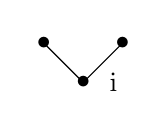
\begin{tikzpicture}[baseline=0cm]
	\node at (0,0)[label=right:{i}]  {$\bullet$};
	\node at (-0.5,0.5) {$\bullet$};
	\node at (0.5,0.5) {$\bullet$};
	\draw (0,0)--(-0.5,0.5);
	\draw (0,0)--(0.5,0.5);
	\end{tikzpicture}
  \end{center}
  
  $b_ic_ic_i \mbox{ or } b_ic_i^2$
  \end{multicols}

\item[\textbf{-}] At all other vertices write  $a_{*-}$ in the sum where $*$ is the label of the vertex's parent and $-$ is a letter not
yet used as a label. \linebreak Label the vertex with $-$.
\begin{multicols}{2}
 \begin{center}
  	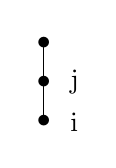
\begin{tikzpicture}[baseline=0cm]
	\node at (0,0)[label=right:{i}]  {$\bullet$};
	\node at (0,0.5)[label=right:{j}]  {$\bullet$};
	\node at (0,1)  {$\bullet$};
	\draw (0,0)--(0,0.5);
	\draw (0,0.5)--(0,1);
	\end{tikzpicture}
  \end{center}
  
  $b_ia_{ij}c_j$
\end{multicols}
\end{itemize}

\section{Deriving the Third Order methods with 3 stages}
First we write out the abstract rooted trees of order $\le 3$ and their corresponding equations
\begin{multicols}{2}
 \begin{center}
  	\begin{tikzpicture}[baseline=0cm]
	\node at (0,-0.7)  {$\bullet$};
	\end{tikzpicture}
  \end{center}

 \begin{center}
  	\begin{tikzpicture}[baseline=0cm]
	\node at (0,0)  {$\bullet$};
	\node at (0,1)  {$\bullet$};
	\draw (0,0)--(0,1);
	\end{tikzpicture}
  \end{center}
\end{multicols}

\begin{multicols}{2}
\begin{center}
$\sum_{i = 1}^s{b_i} = 1$
\end{center}

\begin{center}
$\sum_{i = 1}^s{b_ic_i} = 1/2$
\end{center}
\end{multicols}

\begin{multicols}{2}
 \begin{center}
  	\begin{tikzpicture}[baseline=0cm]
	\node at (0,-1.5)  {$\bullet$};
	\node at (-1,-0.5) {$\bullet$};
	\node at (1,-0.5) {$\bullet$};
	\draw (0,-1.5)--(-1,-0.5);
	\draw (0,-1.5)--(1,-0.5);
	\end{tikzpicture}
  \end{center}

 \begin{center}
  	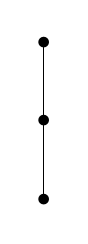
\begin{tikzpicture}[baseline=0cm]
	\node at (0,0)  {$\bullet$};
	\node at (0,1)  {$\bullet$};
	\node at (0,2)  {$\bullet$};
	\draw (0,0)--(0,1);
	\draw (0,1)--(0,2);
	\end{tikzpicture}
  \end{center}
\end{multicols}

\begin{multicols}{2}
\begin{center}
$\sum_{i = 1}^s{b_ic_i^2} = 1/3$
\end{center}

\begin{center}
$\sum_{i = 1}^s{\sum_{j = 1}^{i - 1}{b_ia_{ij}c_j}} = 1/6$
\end{center}
\end{multicols}
\noindent We thus have the system of equations
$$b_1 + b_2 + b_3 = 1$$
$$b_2c_2 + b_3c_3 = 1/2$$
$$b_2c_2^2 + b_3c_3^2 = 1/3$$
$$b_3a_{32}c_2 = 1/6$$
We can now let $c_2$ and $c_3$ be free parameters
in order to make the first three equations into a linear system.
$$\left[ \begin{matrix}
1 & 1 & 1 \\
0 & c_2 & c_3 \\
0 & c_2^2 & c_3^2
\end{matrix} \right] 
\left[ \begin{matrix} 
b_1 \\ b_2 \\ b_3
\end{matrix} \right] = 
\left[ \begin{matrix} 
1 \\ 1/2 \\ 1/3
\end{matrix} \right]$$
and then deal with the fourth equation once $b_1, b_2, b_3$ are known.
The determinant of the coefficient matrix in the linear system is 
$$c_2c_3(c_3 - c_2)$$
There are 3 cases where a solution to the system of equations exists:
\begin{enumerate}
\item[\textbf{Case I}] $$\mathbf{c_2c_3(c_3 - c_2) \ne 0 \mbox{ and } c_2 \ne \frac{2}{3}}$$
The determinant not being 0 gives us a unique solution for $b_1, b_2, b_3$ and implies
$$ b_3 \ne 0 \iff c_2 \ne \frac{2}{3}$$
so a legitimate value for $a_{32}$ will exist if and only if $ c_2 \ne \frac{2}{3}$. \newline \newline
\textbf{Derivation Algorithm for Case I:}
\begin{enumerate}
	\item[1.] Set $c_1 = 0$, choose $c_2, c_3$.
	\item[2.] Solve the linear system to obtain $b_1, b_2, b_3$.
	\item[3.] Set $a_{21} = c_2, a_{32} = \frac{1}{6b_3c_2}, a_{31} = c_3 - a_{32}$. \newline
\end{enumerate}

\item[\textbf{Case II}]
$$\mathbf{c_2 = c_3 = \frac{2}{3}, b_3 \ne 0}$$
If $c_2 = c_3$, then the determinant is $0$ and the equations
$$(b_2 + b_3)c_2 = \frac{1}{2}$$
$$(b_2 + b_3)c_2^2 = \frac{1}{3}$$
must be satisfied. This can only happen if $c_2 = c_3 = \frac{2}{3}$.
We are free to choose values for $b_1, b_2, b_3$ so long as the original 
linear system is satisfied and $b_3$ is not 0
(otherwise a valid value for $a_{32}$ will not exist.) \newline \newline
\textbf{Derivation Algorithm for Case II:}
\begin{enumerate}
	\item[1.] Set $c_1 = 0, c_2 = \frac{2}{3}, c_3 = \frac{2}{3}$.
	\item[2.] Choose $b_3$, set $b_2 = \frac{3}{4} - b_3$, $b_1 = 1 - b_2 - b_3$.
	\item[3.] Set $a_{21} = c_2, a_{32} = \frac{1}{6b_3c_2}, a_{31} = c_3 - a_{32}$. \newline
\end{enumerate}


\item[\textbf{Case III}]
$$\mathbf{c_2 = \frac{2}{3}, c_3 = 0, b_3 \ne 0}$$
This case is similar to Case II except the $b_3$ terms do not appear in the system of two equations. \newline \newline
\textbf{Derivation Algorithm for Case III:}
\begin{enumerate}
	\item[1.] Set $c_1 = 0, c_2 = \frac{2}{3}, c_3 = 0$.
	\item[2.] Choose $b_3$, set $b_2 = \frac{3}{4}$, $b_1 = 1 - b_2 - b_3$. 
	\item[3.] Set $a_{21} = c_2, a_{32} = \frac{1}{6b_3c_2}, a_{31} = c_3 - a_{32}$. \newline
\end{enumerate}
\end{enumerate}


\section{Imposing Simplifying Conditions}
Thus far we have figured out a way to obtain the system of equations that a Runge-Kutta method's 
parameters must satisfy without doing any Taylor expansions.
However, as the order of the methods we wish to derive increases, so does the number of rooted trees
and corresponding equations. 
In fact, the number of rooted trees we must deal with seems to grow exponentially. 
The idea now is to impose simplifying conditions that the parameters will satisfy so that we have 
to worry about less rooted trees.
The reason why certain rooted trees can be eliminated is because by imposing the simplifying conditions,
the trees' equations are automatically satisfied. 

The most obvious simplifying conditions we can impose are the $B(\eta)$ conditions. 
The following rooted trees all have a similar form, that is, they all consist of only a root with leaves.
\begin{multicols}{4}
  \begin{center}
  	\begin{tikzpicture}[baseline=0cm]
	\node at (0,-1)  {$\bullet$};
	\end{tikzpicture}
  \end{center}
 
 \begin{center}
  	\begin{tikzpicture}[baseline=0cm]
	\node at (0,-1)  {$\bullet$};
	\node at (0,0)  {$\bullet$};
	\draw (0,-1)--(0,0);
	\end{tikzpicture}
  \end{center}
  
  \begin{center}
  	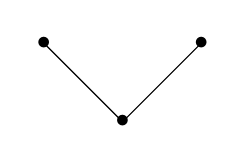
\begin{tikzpicture}[baseline=0cm]
	\node at (-1,0)  {$\bullet$};
	\node at (1,0)  {$\bullet$};
	\node at (0,-1)  {$\bullet$};
	\draw (0,-1)--(-1,0);
	\draw (0,-1)--(1,0);
	\end{tikzpicture}
  \end{center}
  
  \begin{center}
  	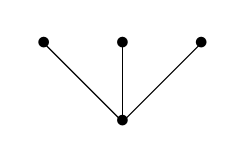
\begin{tikzpicture}[baseline=0cm]
	\node at (-1,0)  {$\bullet$};
	\node at (0,0)  {$\bullet$};
	\node at (1,0)  {$\bullet$};
	\node at (0,-1)  {$\bullet$};
	\draw (0,-1)--(-1,0);
	\draw (0,-1)--(0,0);
	\draw (0,-1)--(1,0);
	\end{tikzpicture}
  \end{center}
\end{multicols}
\noindent For a Runge-Kutta method to have order $p$, we would normally have to worry about $p$ of these trees.
We can instead impose the conditions
$$\sum_{i = 1}^s{b_ic_i^{k - 1}} = 1/k \mbox{ for all } k = 1, 2, \dots, \eta$$
and then set $\eta$ equal to $p$. These are what is meant by the $B(\eta)$
conditions. By specifying ahead of time that these conditions will be imposed,
we can treat the equations for these rooted trees as being satisfied. 

One of the most useful conditions to impose when deriving Runge-Kutta methods of order 4 and above 
is the $D(1)$ condition. Suppose that we have the equations holding for two rooted trees of the form
\begin{multicols}{2}
\begin{center}
  	\begin{tikzpicture}[baseline=0cm]
	\node at (0,0)  {$\bullet$};
	\node at (0,1)  {$*$};
	\draw (0,0)--(0,1);
	\end{tikzpicture}
  \end{center}
 
 \begin{center}
  	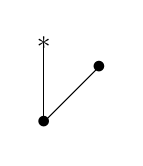
\begin{tikzpicture}[baseline=0cm]
	\node at (0,0)  {$\bullet$};
	\node at (0,1)  {$*$};
	\node at (0.7,0.7)  {$\bullet$};
	\draw (0,0)--(0,1);
	\draw (0,0)--(0.7,0.7);
	\end{tikzpicture}
  \end{center}
\end{multicols}
If the $D(1)$ condition holds, then the equation for the following tree is automatically satisfied
\begin{center}
  	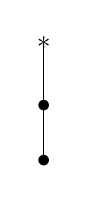
\begin{tikzpicture}[baseline=0cm]
	\node at (0,0.7)  {$\bullet$};
	\node at (0,1.5)  {$*$};
	\node at (0,0)  {$\bullet$};
	\draw (0,0)--(0,0.7);
	\draw (0,0.7)--(0,1.5);
	\end{tikzpicture}
  \end{center}
  Let's call these trees (from left to right) $t_1, t_2, \mbox{ and } t_3$.
  \begin{multicols}{4}
\begin{center}
  	\begin{tikzpicture}[baseline=0cm]
	\node at (0,0)  {$\bullet$};
	\node at (0,1)  {$*$};
	\draw (0,0)--(0,1);
	\end{tikzpicture}
  \end{center}
 
 \begin{center}
  	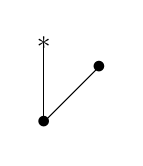
\begin{tikzpicture}[baseline=0cm]
	\node at (0,0)  {$\bullet$};
	\node at (0,1)  {$*$};
	\node at (0.7,0.7)  {$\bullet$};
	\draw (0,0)--(0,1);
	\draw (0,0)--(0.7,0.7);
	\end{tikzpicture}
  \end{center}
  \columnbreak
  \topskip0pt
  \vspace*{\fill}
     \hfill $\Longrightarrow$ \hfill
  \vspace*{\fill}
  \columnbreak
 \begin{center}
  	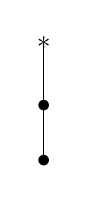
\begin{tikzpicture}[baseline=0cm]
	\node at (0,0.7)  {$\bullet$};
	\node at (0,1.5)  {$*$};
	\node at (0,0)  {$\bullet$};
	\draw (0,0)--(0,0.7);
	\draw (0,0.7)--(0,1.5);
	\end{tikzpicture}
  \end{center}
\end{multicols}
Then in general,
$$\frac{1}{\gamma(t_1)} - \frac{1}{\gamma(t_2)} = \frac{1}{\gamma(t_3)}$$
So we want to force
$$\sum_j{b_i*} - \sum_j{b_ic_j*} = \sum_j\sum_i{b_ia_{ij}*}$$
(Note that we label the roots of $t_1$ and $t_2$ with $j$ instead of $i$ so that it is easier to visualize how the $*$
term can be taken out of the sum. In $t_3$, the $*$ term involves the label for the child of the root, not the root's label.)

The $D(1)$ condition states that 
$$b_i(1 - c_j) = \sum_{i = 1}^s{b_ia_{ij}} \mbox{ for any } j = 1, 2, \dots, s$$ 
In general, the $D(k)$ condition states that (for any $j = 1, 2, \dots, s$)
$$\frac{1}{q}b_i(1 - c_j^q) = \sum_{i = 1}^s{b_i c_i^{q - 1}a_{ij}} \mbox{ for all } q = 1,2, \dots, k$$
but for explicit Runge-Kutta methods, only the $D(1)$ condition can be used since the $D(2)$ condition leads
to an inconsistent system of equations.

Some examples of rooted trees that can be eliminated by imposing the $D(1)$ condition are now given.
Assuming $D(1)$ and the equations for the rooted trees on the left are satisfied, we can ignore the equations
for the rooted trees on the right
\begin{multicols}{4}
  \begin{center}
  	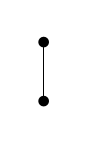
\begin{tikzpicture}[baseline=0cm]
	\node at (0,-0.75)  {$\bullet$};
	\node at (0,0)  {$\bullet$};
	\draw (0,-0.75)--(0,0);
	\end{tikzpicture}
  \end{center}
  \columnbreak
  \begin{center}
  	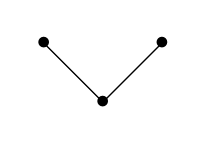
\begin{tikzpicture}[baseline=0cm]
	\node at (0,-0.75)  {$\bullet$};
	\node at (-0.75,0)  {$\bullet$};
	\node at (0.75,0)  {$\bullet$};
	\draw (0,-0.75)--(-0.75,0);
	\draw (0,-0.75)--(0.75,0);
	\end{tikzpicture}
  \end{center}
  \columnbreak
  \topskip0pt
  \vspace*{\fill}
     \hfill $\Longrightarrow$ \hfill
  \vspace*{\fill}
  \columnbreak
  \begin{center}
  	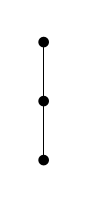
\begin{tikzpicture}[baseline=0cm]
	\node at (0,-0.75)  {$\bullet$};
	\node at (0,0)  {$\bullet$};
	\node at (0,0.75)  {$\bullet$};
	\draw (0,-0.75)--(0,0);
	\draw (0,0)--(0,0.75);
	\end{tikzpicture}
  \end{center}
\end{multicols}
\begin{multicols}{4}
\begin{center}
  	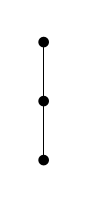
\begin{tikzpicture}[baseline=0cm]
	\node at (0,-0.75)  {$\bullet$};
	\node at (0,0)  {$\bullet$};
	\node at (0,0.75)  {$\bullet$};
	\draw (0,-0.75)--(0,0);
	\draw (0,0)--(0,0.75);
	\end{tikzpicture}
  \end{center}
  \columnbreak
 \begin{center}
  	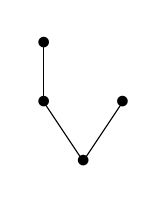
\begin{tikzpicture}[baseline=0cm]
	\node at (0,-0.75)  {$\bullet$};
	\node at (-0.5,0)  {$\bullet$};
	\node at (0.5,0)  {$\bullet$};
	\node at (-0.5,0.75)  {$\bullet$};
	\draw (0,-0.75)--(-0.5,0);
	\draw (0,-0.75)--(0.5,0);
	\draw (-0.5,0)--(-0.5,0.75);
	\end{tikzpicture}
  \end{center}
  \columnbreak
  \topskip0pt
  \vspace*{\fill}
     \hfill $\Longrightarrow$ \hfill
  \vspace*{\fill}
  \columnbreak
  \begin{center}
  	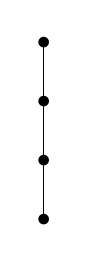
\begin{tikzpicture}[baseline=0cm]
	\node at (0,-0.75)  {$\bullet$};
	\node at (0,0)  {$\bullet$};
	\node at (0,0.75)  {$\bullet$};
	\node at (0,1.5)  {$\bullet$};
	\draw (0,-0.75)--(0,0);
	\draw (0,0)--(0,0.75);
	\draw (0,0.75)--(0,1.5);
	\end{tikzpicture}
  \end{center}
\end{multicols}
\begin{multicols}{4}
  \begin{center}
  	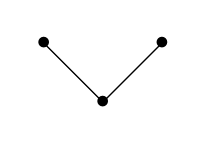
\begin{tikzpicture}[baseline=0cm]
	\node at (0,-0.75)  {$\bullet$};
	\node at (-0.75,0)  {$\bullet$};
	\node at (0.75,0)  {$\bullet$};
	\draw (0,-0.75)--(-0.75,0);
	\draw (0,-0.75)--(0.75,0);
	\end{tikzpicture}
  \end{center}
  \columnbreak
  \begin{center}
  	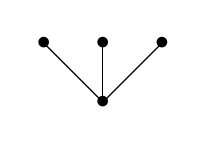
\begin{tikzpicture}[baseline=0cm]
	\node at (0,-0.75)  {$\bullet$};
	\node at (-0.75,0)  {$\bullet$};
	\node at (0,0)  {$\bullet$};
	\node at (0.75,0)  {$\bullet$};
	\draw (0,-0.75)--(-0.75,0);
	\draw (0,-0.75)--(0,0);
	\draw (0,-0.75)--(0.75,0);
	\end{tikzpicture}
  \end{center}
  \columnbreak
   \topskip0pt
  \vspace*{\fill}
     \hfill $\Longrightarrow$ \hfill
  \vspace*{\fill}
  \columnbreak
  \begin{center}
  	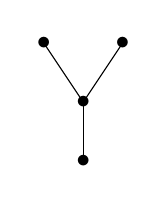
\begin{tikzpicture}[baseline=0cm]
	\node at (0,-0.75)  {$\bullet$};
	\node at (0,0)  {$\bullet$};
	\node at (-0.5,0.75)  {$\bullet$};
	\node at (0.5,0.75)  {$\bullet$};
	\draw (0,-0.75)--(0,0);
	\draw (0,0)--(-0.5,0.75);
	\draw (0,0)--(0.5,0.75);
	\end{tikzpicture}
  \end{center}
\end{multicols}

 \section{Deriving the Fourth Order Methods with 4 Stages} 
 Before writing out the abstract rooted trees with $r(|t|) \le 4$, we are going to decide to
 impose the $B(4)$ and $D(1)$ conditions.
 The $B(4)$ condition takes care of
\begin{multicols}{4}
  \begin{center}
  	\begin{tikzpicture}[baseline=0cm]
	\node at (0,-0.6)  {$\bullet$};
	\end{tikzpicture}
  \end{center}
 
 \begin{center}
  	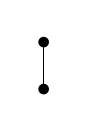
\begin{tikzpicture}[baseline=0cm]
	\node at (0,-0.6)  {$\bullet$};
	\node at (0,0)  {$\bullet$};
	\draw (0,-0.6)--(0,0);
	\end{tikzpicture}
  \end{center}
  
  \begin{center}
  	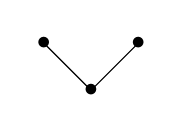
\begin{tikzpicture}[baseline=0cm]
	\node at (-0.6,0)  {$\bullet$};
	\node at (0.6,0)  {$\bullet$};
	\node at (0,-0.6)  {$\bullet$};
	\draw (0,-0.6)--(-0.6,0);
	\draw (0,-0.6)--(0.6,0);
	\end{tikzpicture}
  \end{center}
  
  \begin{center}
  	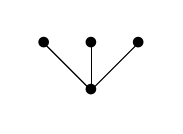
\begin{tikzpicture}[baseline=0cm]
	\node at (-0.6,0)  {$\bullet$};
	\node at (0,0)  {$\bullet$};
	\node at (0.6,0)  {$\bullet$};
	\node at (0,-0.6)  {$\bullet$};
	\draw (0,-0.6)--(-0.6,0);
	\draw (0,-0.6)--(0,0);
	\draw (0,-0.6)--(0.6,0);
	\end{tikzpicture}
  \end{center}
\end{multicols}
The $D(1)$ condition takes care of
\begin{multicols}{3}
\begin{center}
  	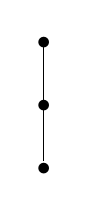
\begin{tikzpicture}[baseline=0cm]
	\node at (0,-1.6)  {$\bullet$};
	\node at (0,-0.8)  {$\bullet$};
	\node at (0,0)  {$\bullet$};
	\draw (0,-1.5)--(0,-0.8);
	\draw (0,-0.8)--(0,0);
	\end{tikzpicture}
  \end{center}
  
\begin{center}
  	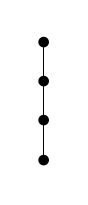
\begin{tikzpicture}[baseline=0cm]
	\node at (0,-1.5)  {$\bullet$};
	\node at (0,-1.0)  {$\bullet$};
	\node at (0,-0.5)  {$\bullet$};
	\node at (0,0)  {$\bullet$};
	\draw (0,-1.5)--(0,-1.0);
	\draw (0,-1.0)--(0,-0.5);
	\draw (0,-0.5)--(0,0);
	\end{tikzpicture}
  \end{center}
  
  \begin{center}
  	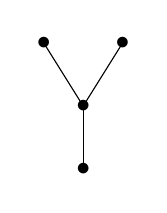
\begin{tikzpicture}[baseline=0cm]
	\node at (0,-1.6)  {$\bullet$};
	\node at (0,-0.8)  {$\bullet$};
	\node at (-0.5,0)  {$\bullet$};
	\node at (0.5,0)  {$\bullet$};
	\draw (0,-1.6)--(0,-0.8);
	\draw (0,-0.8)--(-0.5,0);
	\draw (0,-0.8)--(0.5,0);
	\end{tikzpicture}
  \end{center}
\end{multicols}
What's left?
\begin{center}
  	\begin{tikzpicture}[baseline=0cm]
	\node at (0,-0.75)  {$\bullet$};
	\node at (-0.5,0)  {$\bullet$};
	\node at (0.5,0)  {$\bullet$};
	\node at (-0.5,0.75)  {$\bullet$};
	\draw (0,-0.75)--(-0.5,0);
	\draw (0,-0.75)--(0.5,0);
	\draw (-0.5,0)--(-0.5,0.75);
	\end{tikzpicture}
  \end{center}
 
 It turns out that all fourth order Runge-Kutta methods with four stages have $c_4 = 1$
 (this is shown by \textit{Butcher} and merely involves some manipulation of the rooted tree equations.)
 As a consequence of this, $D(1)$ can be shown to hold for these methods so it makes perfect sense to impose it. To deal with
\begin{multicols}{2}
\begin{center}
  	\begin{tikzpicture}[baseline=0cm]
	\node at (0,-0.75)  {$\bullet$};
	\node at (-0.5,0)  {$\bullet$};
	\node at (0.5,0)  {$\bullet$};
	\node at (-0.5,0.75)  {$\bullet$};
	\draw (0,-0.75)--(-0.5,0);
	\draw (0,-0.75)--(0.5,0);
	\draw (-0.5,0)--(-0.5,0.75);
	\end{tikzpicture}
  \end{center}
  
  $$\sum_{i = 1}^4\sum_{j = 1}^{i - 1}{b_ic_ia_{ij}c_j} = 1/8$$
\end{multicols}
we can subtract it from 
\begin{multicols}{2}
\begin{center}
  	\begin{tikzpicture}[baseline=0cm]
	\node at (0,-1.6)  {$\bullet$};
	\node at (0,-0.8)  {$\bullet$};
	\node at (0,0)  {$\bullet$};
	\draw (0,-1.5)--(0,-0.8);
	\draw (0,-0.8)--(0,0);
	\end{tikzpicture}
  \end{center}
  
  $$\sum_{i = 1}^4\sum_{j = 1}^{i - 1}{b_ia_{ij}c_j} = 1/6$$
\end{multicols}
\noindent to get the more convenient equation
$$(\sum_{i = 1}^4\sum_{j = 1}^{i - 1}{b_i(1 - c_i)a_{ij}c_j} =) \mbox{ } b_3(1 - c_3)a_{32}c_2 = 1/24$$
We thus have the system of equations
$$\sum_{i = 1}^4{b_ic_i^{k - 1}} = 1/k \mbox{ for all } k = 1, 2, \dots, 4$$
$$b_i(1 - c_j) = \sum_{i = 1}^4{b_ia_{ij}} \mbox{ for all } j = 1, 2, \dots, 4$$ \newline
$$b_3(1 - c_3)a_{32}c_2 = 1/24$$
A general approach to constructing 4-stage methods of order 4 is:
\begin{enumerate}
\item[1.] Choose values for $c_2$ and $c_3$, noting that $c_1 = 0$ and $c_4 = 1$.
\item[2.] Obtain $b_1, b_2, b_3, b_4$ by solving the linear system
$$\sum_{i = 1}^4{b_ic_i^{k - 1}} = 1/k \mbox{ for all } k = 1, 2, \dots, 4$$
\item[3.] Set $a_{32} = \frac{1}{24b_3(1 - c_3)c_2}, a_{31} = c_3 - a_{32}, a_{21} = c_2$. 
\item[4.] Obtain $a_{41}, a_{42}, a_{43}$ by using the $D(1)$ equations
$$a_{4j} = \frac{b_i(1 - c_j) - \sum_{i = 1}^{3}{b_ia_{ij}}}{b_4} \mbox{ for } j = 1, 2, 3$$
\end{enumerate}
As with the third order methods, there are some values for free parameters that will not lead to a
solution to the system of equations. According to \textit{Butcher}, Kutta identified five cases where a solution
is certain to exist:
\begin{itemize}
\item[I]$$c_2 \notin \{ 0, \frac12, \frac12 \pm \frac{\sqrt3}{6}, 1\}, c_3 = 1 - c_2$$
\item[II] $$b_2 = 0, c_2 \ne 0, c_3 = \frac12$$
\item[III] $$b_3 \ne 0, c_2 \ne \frac12, c_3 = 0$$
\item[IV] $$b_4 \ne 0, c_2 = 1, c_3 = \frac12$$
\item[V] $$b_3 \ne 0, c_2 = c_3 = \frac12$$
\end{itemize}

\section{Obtaining the Efficient Frontier}
In the financial world, an efficient portfolio is a portfolio that has the minimum risk for a given level
of expected return or the highest expected return for a given level of risk. When modelling portfolios
using probability, the variance of the portfolio is used to estimate how risky it is.

\textit{Yao, Lai, and Li} showed that in a model where the assets and liabilities
take on values determined by an $m$-dimensional Brownian motion and where the liabilities are endogenous
(that is, the liabilities can be controlled, e.g. a company issuing bonds)
the efficient frontier can be obtained by solving the ODEs
$$\Omega'(t) + A(t)\Omega(t) + \Omega(t)A(t) + \sum_{j=1}^m{C_j(t)\Omega(t)C_j(t)} - 
\left(\Omega(t)B(t) + \sum_{j=1}^m{C_j(t)\Omega(t)D_j(t)}\right)$$
$$\cdot \left( \sum_{j=1}^m{D_j^T(t)\Omega(t)D_j(t)} \right)^{-1}
\left( B^T(t)\Omega(t) + \sum_{j=1}^m{D_j^T(t)\Omega(t)C_j(t)} \right) = 0$$ \newline
$$g'(t) + \left( A(t) - \left( \Omega(t)B(t) + \sum_{j=1}^m{C_j(t)\Omega(t)D_j(t)} \right) 
\cdot \left( \sum_{j=1}^m{D_j^T(t)\Omega(t)D_j(t)} \right)^{-1} B^T(t)\right)g(t) = 0$$ \newline
$$\varphi'(t) - \frac{1}{4}g^T(t)B(t)\left( \sum_{j=1}^m{D_j^T(t)\Omega(t)D_j(t)} \right)^{-1} B^T(t)g(t) = 0$$ \newline
for $\Omega(t), g(t),$ and $\varphi(t)$ subject to the terminal conditions
$$\Omega(T_0) = \left( \begin{array}{c c} 
1 & -1 \\
-1 & 1
\end{array} \right), 
g(T_0) =  \left( \begin{array}{c} 
2 \\
-2 
\end{array} \right),
\varphi(T_0) = 0$$
where $\Omega(t)$ is a $2 \times 2$ matrix-valued function, $g(t)$ is a $2 \times 1$ vector-valued function,
and $\varphi(t)$ is a scalar-valued function. Here $T_0$ is the end of the investment period (denoted $T$
in the original article,) and $A(t), B(t), C_j(t), D_j(t) \mbox{ (where } j = 1,2, \dots, m)$ are market parameters.

We wish to find the efficient frontier for portfolios at time $T_n < T_0$.  
For a given expected return $d$, the corresponding minimum variance is
$$-\frac{1 + \varphi(T_n)}{\varphi(T_n)}\left( d - \frac{g^T(T_n)z_{T_n}}{2(1 + \varphi(T_n))} \right)^2
+ z_{T_n}^T\left(\Omega(T_n) - \frac{g(T_n)g^T(T_n)}{4(1 + \varphi(T_n))}\right)z_{T_n}$$
Here $z_{T_n}$ is the current difference between the value of all assets and the value of all liabilities
at time $T_n$ (the surplus at time $T_n$). The article also includes an expression for the portfolio that gives us this variance.

The article concluded with some numerical examples including one where the efficient frontier was
found for a model with initial surplus $1$, initial time $0$, final time $5$, two assets, two liabilities and parameters
$$A(t) = \left( \begin{array}{c c} 
0.0161 & 0 \\
0 & 0.0153
\end{array} \right),
B(t) = \left( \begin{array}{c c} 
0.0068 & 0 \\
0 & -0.0064
\end{array} \right),$$
$$
L(t)Y^T(t) = \left( \begin{array}{c c} 
-0.0528 & -0.0119 \\
0.0014 & -0.0812
\end{array} \right),
L(t)L^T(t) = \left( \begin{array}{c c} 
0.0923 & 0.0402 \\
0.0402 & 0.1080
\end{array} \right),
$$
$$
Y(t)Y^T(t) = \left( \begin{array}{c c} 
0.0978 & -0.0040 \\
-0.0040 & 0.1468
\end{array} \right)
$$
where the bottom 3 matrices are related to the $C_j$ and $D_j$ market parameters.
\textit{Yao, Lai, and Li} obtained the frontier for this example numerically by applying a variation 
of the RK4 Runge-Kutta method with $N = 45$ subintervals using Matlab. 
The author of the current paper you are reading reproduced their results for this example
using Maple. 

The efficient frontier for the example thus looks like
\begin{figure}[!htb]
   \centering
   \includegraphics[width = \textwidth, height = 0.5\textheight]{./"images/frontier"}
 \end{figure}
 
 \pagebreak



   


\section{Some Discussion of Stability}
When it comes to numerical algorithms for solving ODEs, the term stability refers to how well
the algorithm performs as the distance to the endpoint we wish to approximate $y(x)$ at 
becomes larger and larger. As a motivating example, consider the initial value problem
$$y'(x) = qy(x) \mbox{ with } y(0) = 1 \mbox{ where } q < 0$$
The solution to this problem is 
$$y(x) = e^{qx}$$
and we see that $y \rightarrow 0$ as $x \rightarrow \infty$.

If we apply the Euler method to this problem, then
$$y_{n + 1} = y_n + hf(y_n) = y_n + hqy_n = (1 + hq)y_n$$
Thus
$$y_n = (1 + hq)^ny_0$$
If $h$ is too big, then the Euler method will not have the desired property of having the
approximation go to $0$. The region of values for $h$ that give us the desired behaviour depends
on what $q$ is. Letting $z = hq$, the stability region for the Euler method is defined as the set of complex
numbers $z$ such that $y_n$ remains bounded even as $n \to \infty$.
($z$ is complex since this discussion also applies to linear ODEs involving matrices with complex eigenvalues.)

For the example, the stability region is
$$\{z \in \mathbb{C} : |1 + z| \le 1\}$$

We are interested in what happens when $z$ is negative since in this case we know that the exact solution
remains bounded.
\begin{definition}
A numerical method is said to be \textbf{A-stable} if for the initial value problem
$$y'(x) = qy(x) \mbox{ with } y(0) = 1 \mbox{ where } Re(q) < 0$$
(where $h$ is assumed to be fixed,)
the computed approximation $y_n$ remains bounded as $n \to \infty$.
\end{definition}
\begin{theorem}
Explicit Runge-Kutta methods are not A-stable.
\end{theorem}
This result is shown by recognizing that in the case of a Runge-Kutta method, we can write
$$y_n = \phi(hq)^ny_0$$
where $\phi(z)$ is known as the stability function. For explicit Runge-Kutta methods, $\phi(z)$
turns out to be a polynomial and thus the explicit methods are not A-stable.
There do however exist implicit Runge-Kutta methods (such as the implicit Euler method)
that are A-stable. Moreover, the rooted tree approach of deriving Runge-Kutta methods still works
when deriving implicit methods (in fact, there are more simplifying conditions that can be imposed
in the implicit case.)
\pagebreak

\section{Conclusion}
This concludes the project of figuring out (with proof) how to derive the explicit Runge-Kutta methods using rooted trees.
The Butcher group was not explored but the mechanics behind a very interesting approach to solving a problem
in numerical analysis were learned. In addition, Runge-Kutta was seen in action when applied to a problem in financial
math that appeared in a very recent article (2013). The discussion of stability is relevant  if one wishes to use Runge-Kutta
methods to numerically solve a so-called stiff problem. 

\section[*]{References}
  \begin{itemize} \item Butcher, John C., \textit{Numerical Methods for Ordinary Differential   
  Equations} (2008), second edition,
  \item Nagle et al., \textit{Fundamentals of Differential Equations and Boundary Value Problems}
           (2012), sections 3.6 and 3.7, sixth edition,
  \item Matthews, John H. and Fink, Kurtis D., \textit{Numerical Methods using Matlab} (2004),
           sections 9.4 and 9.5, fourth edition, 
  \item Yao, Haixiang; Lai, Yongzeng; Li, Yong; \textit{Continuous-time mean-variance asset-liability management
  with endogenous liabilities} (2013), ScienceDirect, Insurance: Mathematics and Economics, Volume 52, Issue 1.
  \end{itemize}
\end{document}